\chapter{Modelling object lifetimes in finite networks under churn}
\label{chp:MODELLING}

To increase the time an object is available within a distributed storage system, two techniques are used: redundancy and repair. In storage systems using replication as redundancy technique, $R$ replicas of every object are stored. The number of required replicas $R$ is a design decision, the effect of which will be shown in Section \ref{results}. When all nodes containing an object's replicas have left the network, the object is no longer available. Periodic repair, which occurs at a rate of $\mu = 1/T_{\textrm{repair}}$, replaces all missing replicas.

\section{Related work}
\label{model_related_work}

This chapter mainly extends and improves upon the work by Wu, Tian and Ng \cite{replication_article}. The related work models three characteristics of distributed hash table (DHT) lookups under churn: expected lookup latency of various routing schemes, expected lookup overhead of various routing schemes and expected object lifetime. We focus on the object lifetime characteristic. Wu, Tian and Ng develop two models for object lifetime when exponentially distributed node lifetimes are assumed. One for the case without object repair and one for the case with object repair. Node residual lifetimes are used when calculating expected object lifetimes without repair. In this case object lifetimes are equal to the maximum residual lifetime of the nodes the objects were replicated on.

%What about Pareto lifetimes?

A continuous time Markov chain, shown in Figure \ref{fig_other_markov_chain}, is used to model the expected object lifetimes for the case with repair.
%
\begin{figure}[htbp]
 \centering
 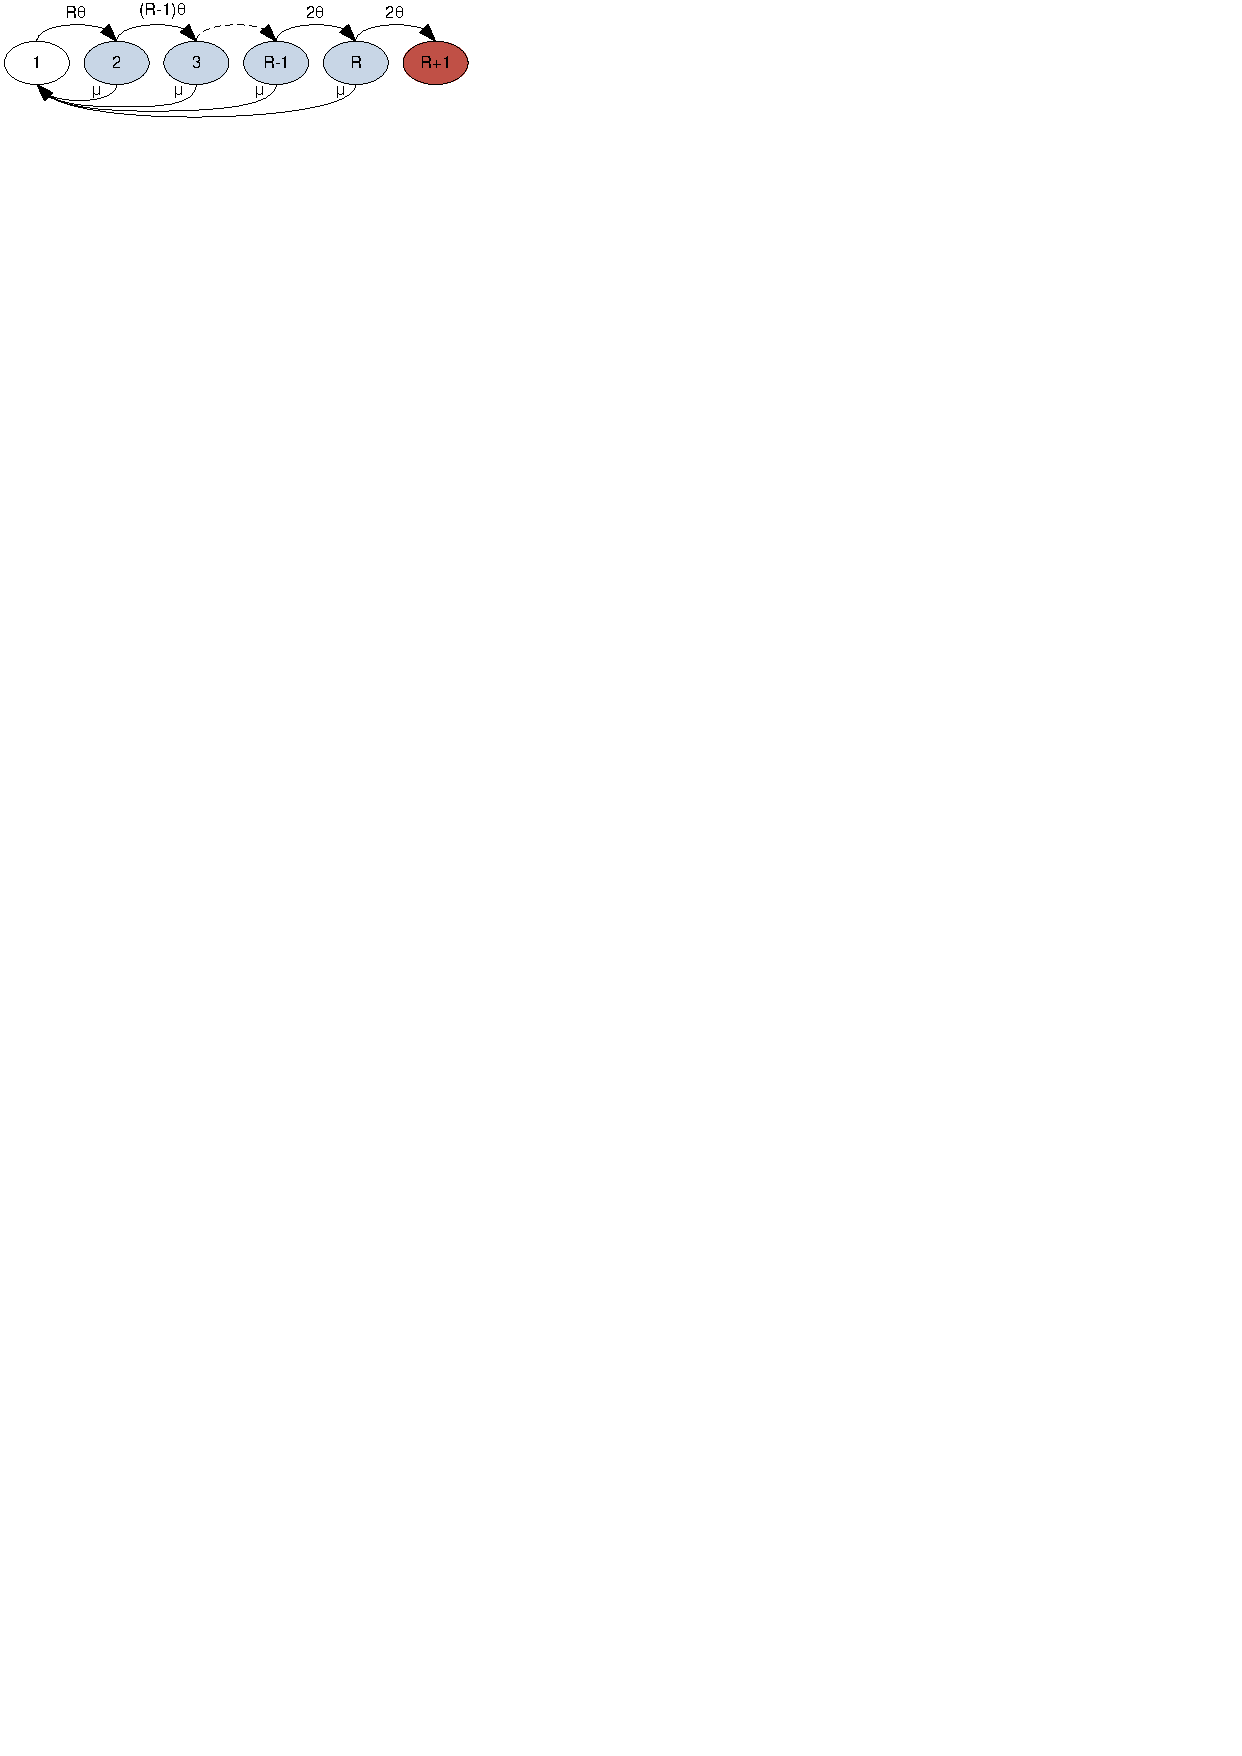
\includegraphics[clip=true, viewport=0.0cm 27.5cm 8.0cm 30.0cm, width=0.7\columnwidth]{inifinite_network_chain}
 \caption{Markov chain modeling object replica number for an infinite network size}
 \label{fig_other_markov_chain}
\end{figure}
%
The model has $R+1$ states and is in state $k$ when $R+1-k$ replicas are alive in the network. The system is, therefore, in state $1$ when all replicas are present and in state $R+1$ when no replicas are present. The authors assume that all objects are inserted into the network with $R$ replicas, i.e. enter the network in state 1. This initial state is colored white in Figure \ref{fig_other_markov_chain}. If the node departure rate under steady state is $\theta$ and there are $r$ replicas present in the network, the replica departure rate under steady state is $r\theta$. When all replicas are lost, the chain enters state $R+1$ (coloured dark) and is said to be ``absorbed''.

In this chapter, we improve on the work by Wu, Tian and Ng \cite{replication_article} in two ways: firstly, the model is extended to take into account a finite network size. The fact that there might not be sufficient nodes to replicate the data on when objects are stored or when the repair mechanism activates. Secondly, our model unifies the cases with and without repair, to produce a single model where the effects of both might be evaluated. When our model is used with larger average network sizes, expected object lifetimes converge to those shown in the work by Wu, Tian and Ng, using their two separate models.

Predicting object lifetimes in a distributed storage system is grounded in reliability engineering theory. When network size is ignored, it is similar to predicting the mean time to failure (MTTF) of a set of parallel components with repair. Chun et al. \cite{Chun:2006_replica_maintenance} also uses a Markov chain to model object replicas with network churn and repair. They use a birth-death process similar to the model by Wu, Tian and Ng, but using incremental, instead of complete repair.

No literature could be found in general reliability engineering or distributed systems reliability research that deals with object lifetimes with finite network sizes.

\section{The model}
\label{model}

In order to model the effects of a finite network size on the lifetime of an object, the continuous time Markov chain model introduced in Section \ref{model_related_work} is expanded by adding a second parameter to every state, namely the network size. This effectively adds another dimension to the Markov chain. The resulting Markov chain is shown in Figure \ref{fig_markov_chain}.

\begin{figure}[htbp]
 \centering
 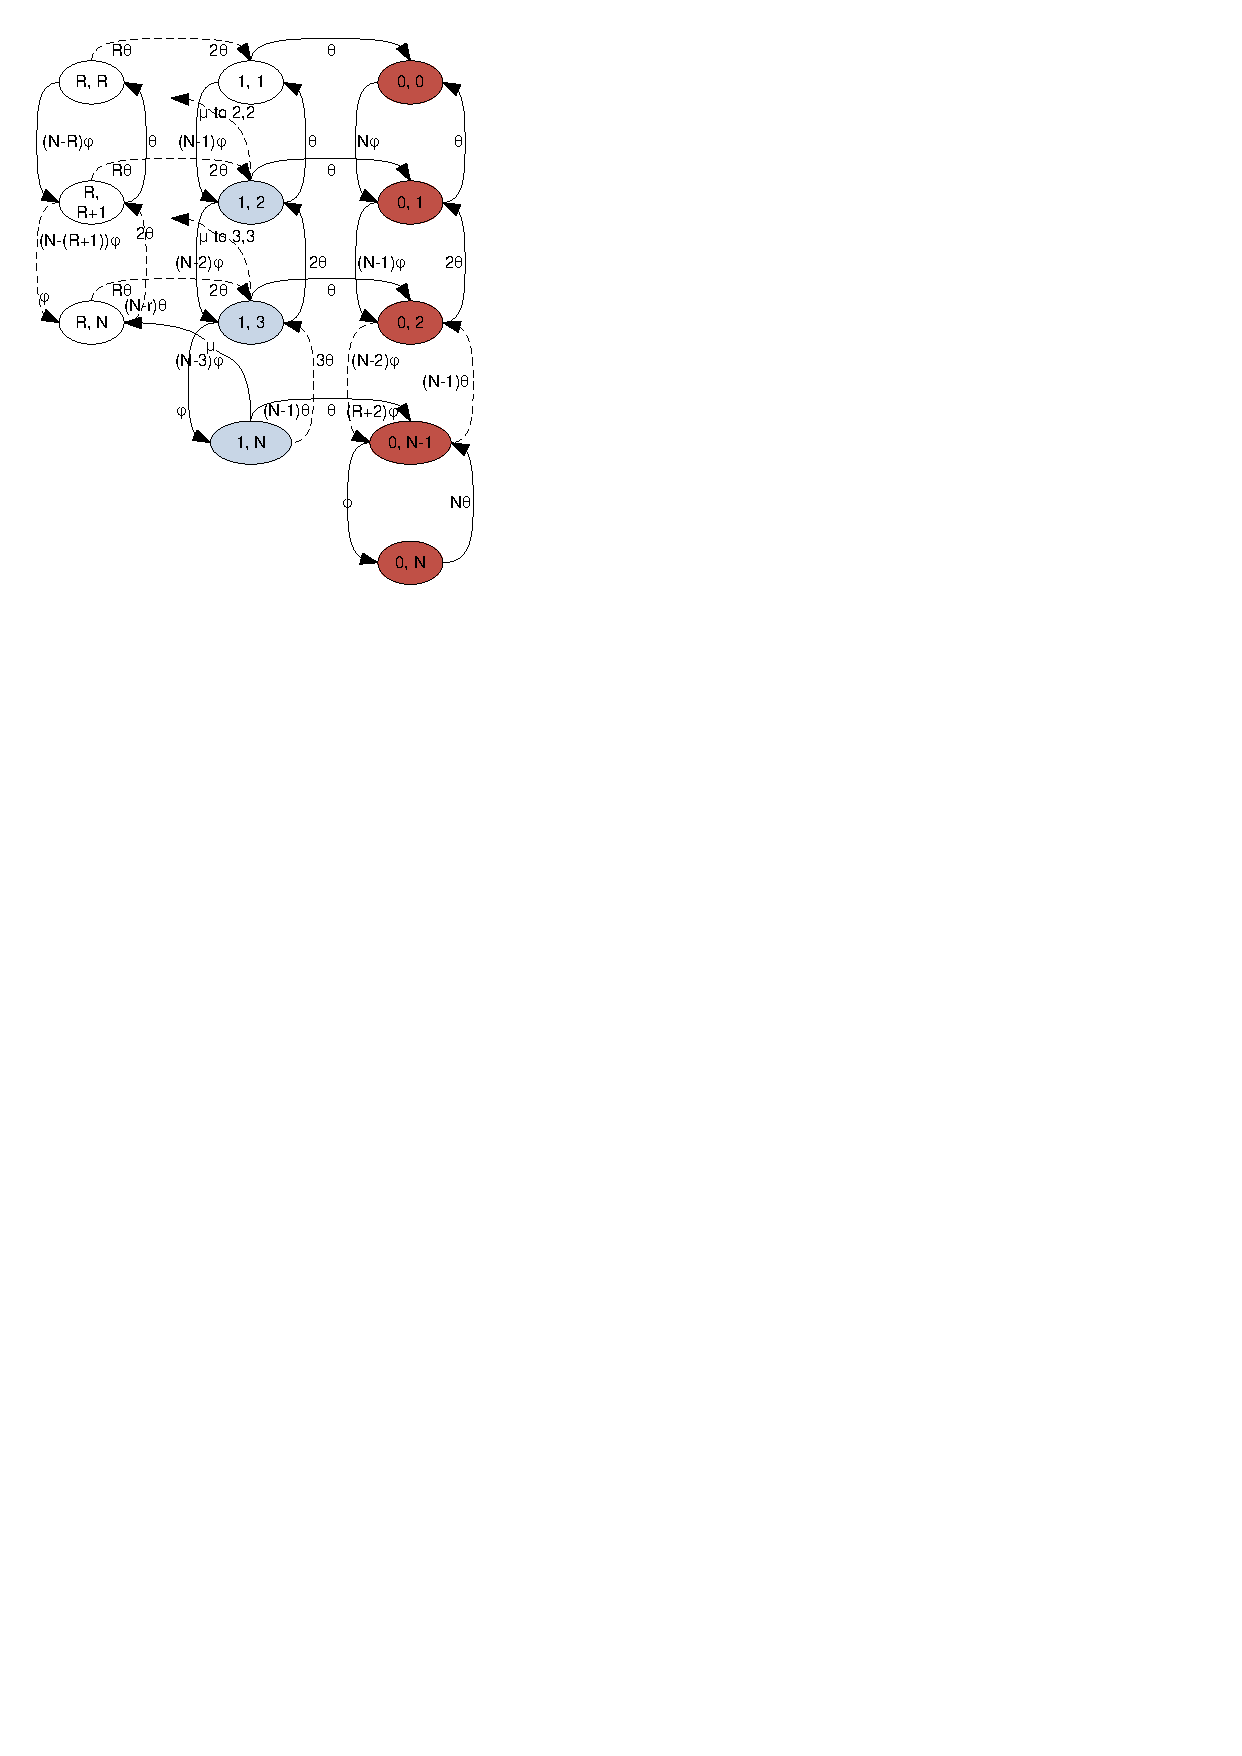
\includegraphics[clip=true, viewport=0.5cm 19.5cm 8.5cm 29.5cm, width=0.7\columnwidth]{Markov_chain_repair_compact}
 \caption{Markov chain modeling object replica number as well as network size}
 \label{fig_markov_chain}
\end{figure}

%Explain transient and absorbtion states here somewhere.

The dual parameter states can be seen in the Markov chain in Figure \ref{fig_markov_chain}. Every state is a tuple of the form \verb.(replicas,nodes).. Where $R$ is the required number of object replicas and $N$ is the maximum number of nodes in the network. It is assumed that $R$ replicas are always stored in the network, if sufficient space is available. If the number of nodes currently in the network $n$ are fewer than the required number of replicas ($n < R$), only $n$ replicas are stored. The initial states of the Markov chain are therefore all the states ($R,n$) as well as all the states ($n,n$), for $n < R$. There are therefore $N$ initial states, one for every possible network size. The initial state is the initial network size that an object is placed in.

If there are no more replicas in the network, an object cannot be repaired and the Markov chains remains in the set of states ($0,n$). These are said to be the absorbing states of the Markov chain and there exists $N - R + 1$ absorbing states in the model presented here. All other states out of which transition is possible are said to be transient states. It can be shown that if sets of transient and absorbing states exist, the system will always end up in the absorbing states \cite{grinstead1997introduction_probability}. The time to absorbtion can be calculated, which in the case of object storage means the time when no more objects exist in the network.

\subsection{State transition rates}

There are four types of state transitions possible in the Markov model presented here:
%
\begin{enumerate}
\item A node that contains a replica departs the network.
\item A node that does not contain a replica departs the network.
\item A node joins the network.
\item An object is repaired.
\end{enumerate}

%In a continous Markov chain we define delta small enough so only one event can occur at any point in time

\begin{figure}[htbp]
 \centering
 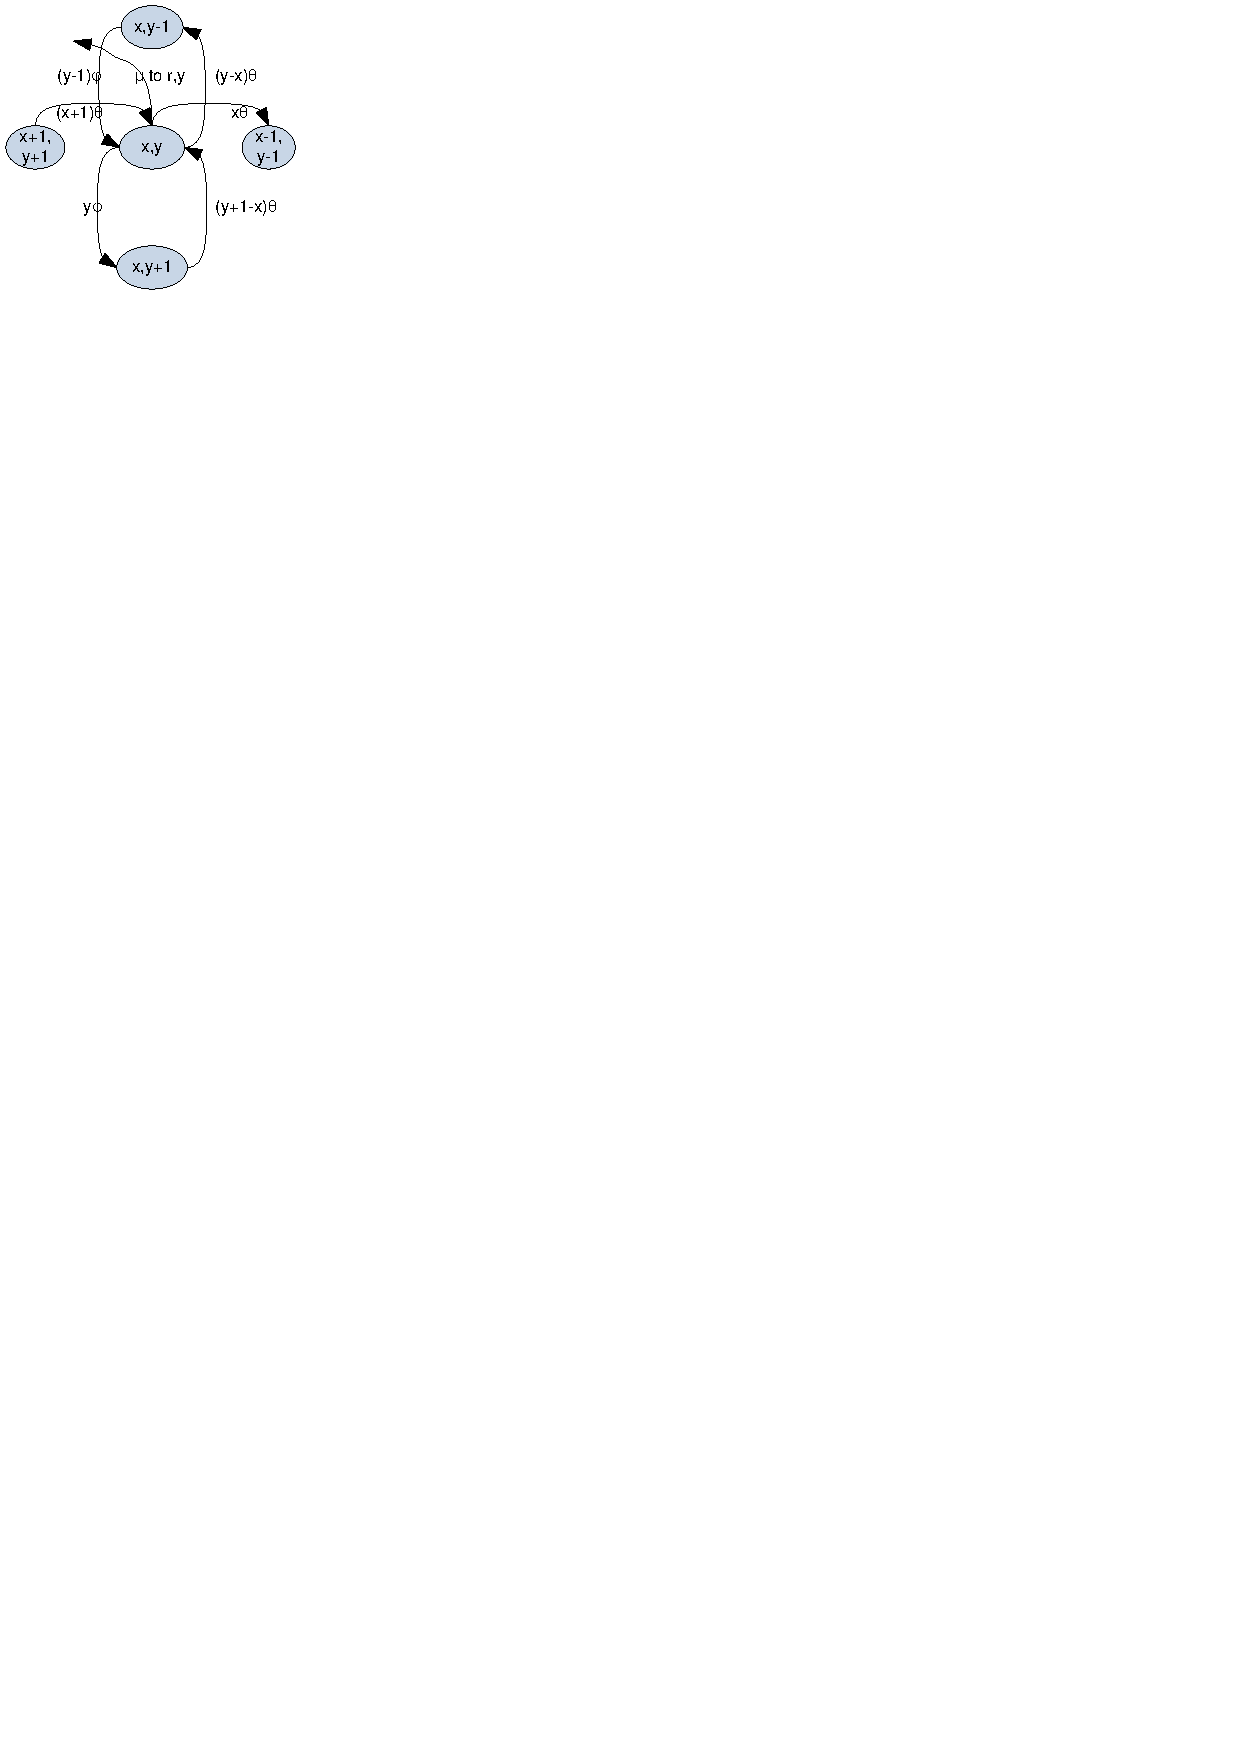
\includegraphics[clip=true, viewport=0.0cm 24.5cm 5.0cm 30cm, width=0.6\columnwidth]{Markov_example}
 \caption{Markov chain modeling object replica number as well as network size}
 \label{fig_markov_example}
\end{figure}

State transitions can be explained by the example in Figure \ref{fig_markov_example}. The figure shows all state transitions relative to the centre state ($i,k$). For the purposes of explanation, only transitions to and from the centre state are shown. Starting at state ($i+1,k+1$), where $i+1$ replicas and $k+1$ nodes are present. If a node that contains a replica departs the network, the system moves to state ($i,k$): one fewer replica and one fewer node.

If a node that does not contain a replica now departs from the network, the system moves from state ($i,k$) to ($i,k-1$): no fewer replicas and one fewer node. A node can join the network, which will have the model move from ($i,k-1$) to ($i,k$) and another node joining the network will move the system into state ($i,k+1$).

The periodic repair mechanism, introduced in Section \ref{model_related_work} is also present. With sufficient nodes available for a full repair, the system moves from state ($i,k$) to ($R,k$). When the network size is smaller than the required number of replicas, the system moves to state ($N,k$) instead.

For dual states, state transition rates are characterised by moving from state $i k$ to state $j l$, where $i$ is the number of replicas in the current state, $k$ the number of nodes in the current state, $j$ the number of replicas in the next state, and $l$ the number of nodes in the next state. Every state transition rate can then be expressed as a dual state transition equation.

Let $\theta$ be the departure rate of nodes under steady state. For a current state of $i$ replicas, the departure rate of nodes containing replicas from the network is $i\theta$. This transition can be expressed in terms of the dual state transition equation:
%
\begin{equation} \label{eq_rep_left}
    p(i k,j l)_{(\textrm{replica left})} = i\theta,\quad\textrm{for}\quad j = i - 1,\quad l = k - 1,
\end{equation}
%
where the next state contains one fewer replica and one fewer node than the current state.

The departure rate of nodes not containing replicas is the difference between the number of nodes currently in the network $k$ and the number of replicas currently in the network $i$. The departure rate is then $(k - i)\theta$ and the transition is given by
%
\begin{equation} \label{eq_node_left}
    p(i k,j l)_{(\textrm{node left})} = (k - i)\theta,\quad\textrm{for}\quad j = i,\quad l = k - 1,
\end{equation}
%
where the next state contains one fewer node, but the same number of replicas as the current state.

The Markov model assumes the presence of a finite sized network, with some maximum number of nodes $N$. Let $\phi$ be the arrival rate of peers under steady state. The departure rate of nodes from the network is dependant on the number of nodes in the network. Similarly, if a maximum network size is assumed, the arrival rate of nodes in the network can be modelled as a function of nodes \emph{not} in the network. This creates a symmetry between the network departure and arrival rates, which creates a ``force'' in the Markov model that pushes the network to some average network size, which is a ratio of $\theta$ to $\phi$. A stationary average network size is required to model a steady state network.

The arrival rate of nodes can thus be modelled as $(N - k)\phi$, the product of a single node arrival rate and the number of nodes not currently in the network, as given by
%
\begin{equation} \label{eq_node_arrived}
    p(i k,j l)_{(\textrm{node arrived})} = (N - k)\phi,\quad\textrm{for}\quad j = i,\quad l = k + 1,
\end{equation}
%
where the next state contains one more node, but the same number of replicas as the current state.

%Perhaps add some graphs here to show how node departure and arrival rate change with changes in network size. Show a graph or equation that will show the trend towards a single average. Perhaps use something like the rate difference to show force towards the centre.

$N$ should be chosen sufficiently large, compared to the average network size $\tilde{n}$, to ensure that the probability of the network model ever reaching $N$ is vanishingly small. What constitutes a sufficiently large maximum network size will be evident from the results presented in Section \ref{results}. This requires that the ratios of $\theta$ to $\phi$ be chosen to produce a network with an average network size much smaller than $N$.

For the network to be in steady state, the mean arrival rate of nodes must equal the mean departure rate of nodes, which gives
%
\begin{equation}
    (N - \tilde{n})\phi = \tilde{n}\theta.\label{eq_phi_theta_ratio}
\end{equation}

Making $\phi$ the subject of Equation \eqref{eq_phi_theta_ratio} gives
%
\begin{equation}
    \phi = \frac{\tilde{n}\theta}{N - \tilde{n}},\label{eq_phi}
\end{equation}
%
which provides a value for $\phi$ that will produce a network with the desired average network size $\tilde{n}$, for a given $\theta$ and $N$.

It is assumed that the repair mechanism repairs objects once every $T_{\textrm{repair}}$ time or at a rate of $\mu = 1/T_{\textrm{repair}}$, which gives
%
\begin{equation} \label{eq_repair}
    p(i k,j l)_{(\textrm{repair})} = \mu,\quad\textrm{for}\quad j = \min(R, l),\quad l = k,\quad i \neq j.
\end{equation}
%
The number of replicas in the next state is either equal to the required number of replicas or the current number of nodes, whichever one is smallest, and the number of nodes remain the same as in the current state. When no replicas are missing, no repair occurs.

No transitions other than the ones described above can occur in the presented Markov model, therefore $p(i k,j l) = 0$ for all other state transitions.

\subsection{Node departure rate}
\label{node_departure_rate}

The node departure rate $\theta$ can be calculated from the lifetime distributions of the nodes in the network. As in the related work discussed in Section \ref{model_related_work}, all node lifetimes are assumed to be statistically independent and exponentially distributed. The exponential distribution is characterised by the single ``rate'' parameter $\lambda$.

The departure rate of nodes correspond to the failure rate (also called the hazard rate) of the node lifetime distribution \cite{rausand2004systemreliability}. An advantage of the exponential distribution is its ``memoryless'' property, which has a constant failure rate $h = \lambda$. For nodes with exponential lifetime distributions, the node departure rate is therefore $\theta = \lambda$.

\subsection{Number of states}

The Markov model presented, possesses a large number of states. To calculate the total number of states, two cases are identified. The first case is where the number of nodes in the network is greater or equal to the required number of replicas $k \geq R$. For every possible network size in this group, there are $R$ states and $N - R + 1$ possible network sizes. From this it is evident that there are $(N - R + 1)R$ of these states.

The second case is where the number of nodes in the network is fewer than the required number of replicas. For every possible network size in this case, the number of states are equal to the number of nodes in the network, going from $R-1$ to 1.

The total number of states is the sum the two cases and given by
%
\begin{align}
       S & = R(N - R + 1) + \sum_{x=1}^{R-1} x\label{eq_states_num_init}\\
         & = R(N - R + 1) + 0.5 (R - 1) R\notag\\
         & = 0.5 R (2 N - R + 1), \quad\textrm{where}\quad N \geq R. \label{eq_states_num_ans}
\end{align}

If a small network of 500 nodes with objects each having 10 replicas is modeled, the resulting Markov chain contains 4955 states. The large number of states makes a closed form solution to the object lifetime problem intractable. Fortunately, numerical methods can be used to calculate object lifetimes for given numbers of replicas and maximum node sizes.

\subsection{Calculating object lifetimes}

Since each element in the transitional rates matrix is a rate, the sum of all the elements in a single row of the rates matrix gives the rate of moving from that state to any other state. The inverse of this rate is the expected time $t_i$ the Markov chain spends in state $i$, given by
%
\begin{equation} \label{eq_markov_rates}
    t_i = \left(\sum_{j} p_{i, j}\right)^{-1}.
\end{equation}

In a embedded Markov chain, the sum of all rows in the transitional rates matrix must equal one. This is achieved by normalising each row in the transitional rates matrix \textbf{P} to produce the normalised transitional rates matrix \textbf{\^{P}}, where each row in the matrix must satisfy
%
\begin{equation} \label{eq_markov_sum}
    \sum_{j} \hat{p}_{i, j} = 1.
\end{equation}

Using $t_i$, the expected time spent in state $i$, \textbf{\^{P}} is given by
%
\begin{equation} \label{eq_markov_normalisation}
    \hat{p}_{i, j} = p_{i, j} t_i.
\end{equation}

Object lifetime can be calculated by calculating the expected time to absorbtion of the embedded continuous time Markov chain. To do this, the normalised transitional rates matrix is partitioned into the form
%
\begin{equation} \label{matrix_partition}
    \textbf{\^{P}} = \left[\begin{array}{c|c}
                   \textbf{Q} & \textbf{R} \\
                   \hline
                   \textbf{0} & \textbf{I}
                 \end{array}\right].
\end{equation}
%
Every state transition can be considered a discrete event, which allows for the continuous time Markov chain to be embedded. This allows for theory from discrete time Markov chains to be used, with the exception that events are not equally spaced in time.

\textbf{\^{P}} is partitioned in such a way that all absorbing states are in the last rows and columns of \textbf{\^{P}}. Suppose there are $a$ absorbing states and $\tau$ transient states in the model. The matrix \textbf{Q} is then a $\tau\times\tau$ sub-matrix of \textbf{\^{P}} that contains all transient states. \textbf{I} is an $a \times a$ identity matrix, \textbf{0} is a $a\times\tau$ zero matrix and \textbf{R} (not to be confused with $R$) is a nonzero $\tau\times a$ matrix.

From \textbf{Q}, the fundamental matrix \textbf{N} may be calculated as \cite{grinstead1997introduction_probability}
%
\begin{equation} \label{eq_fundamental_mat}
    \textbf{N} = (\textbf{I} - \textbf{Q})^{-1}.
\end{equation}
%
Every element $n_{x,y}$ in the fundamental matrix \textbf{N} gives the expected number of times that the model is in the state $y$, if it started in the transient state $x$.

The expected time to absorbtion is then the product of the time spent in each state and the expected number of times a state will be entered, as given by
%
\begin{equation} \label{expected_lifetime}
    \textbf{E[L]} = \textbf{Nt},
\end{equation}
%
where \textbf{t} is the vector consisting of the times $t_i$ for all $i$.

\section{Model results}
\label{results}

For all results presented in this section, the following parameter values are used: a maximum network size of $N=120$, a required number of replicas of $R = 10$ and exponential node lifetime distributions with $\lambda = \theta = 1/1800$, which gives expected \emph{node} lifetimes of $1/\lambda = 1800$ seconds.

%Maybe explain where these values come from or why the were used.

\begin{figure}[htbp]
 \centering
 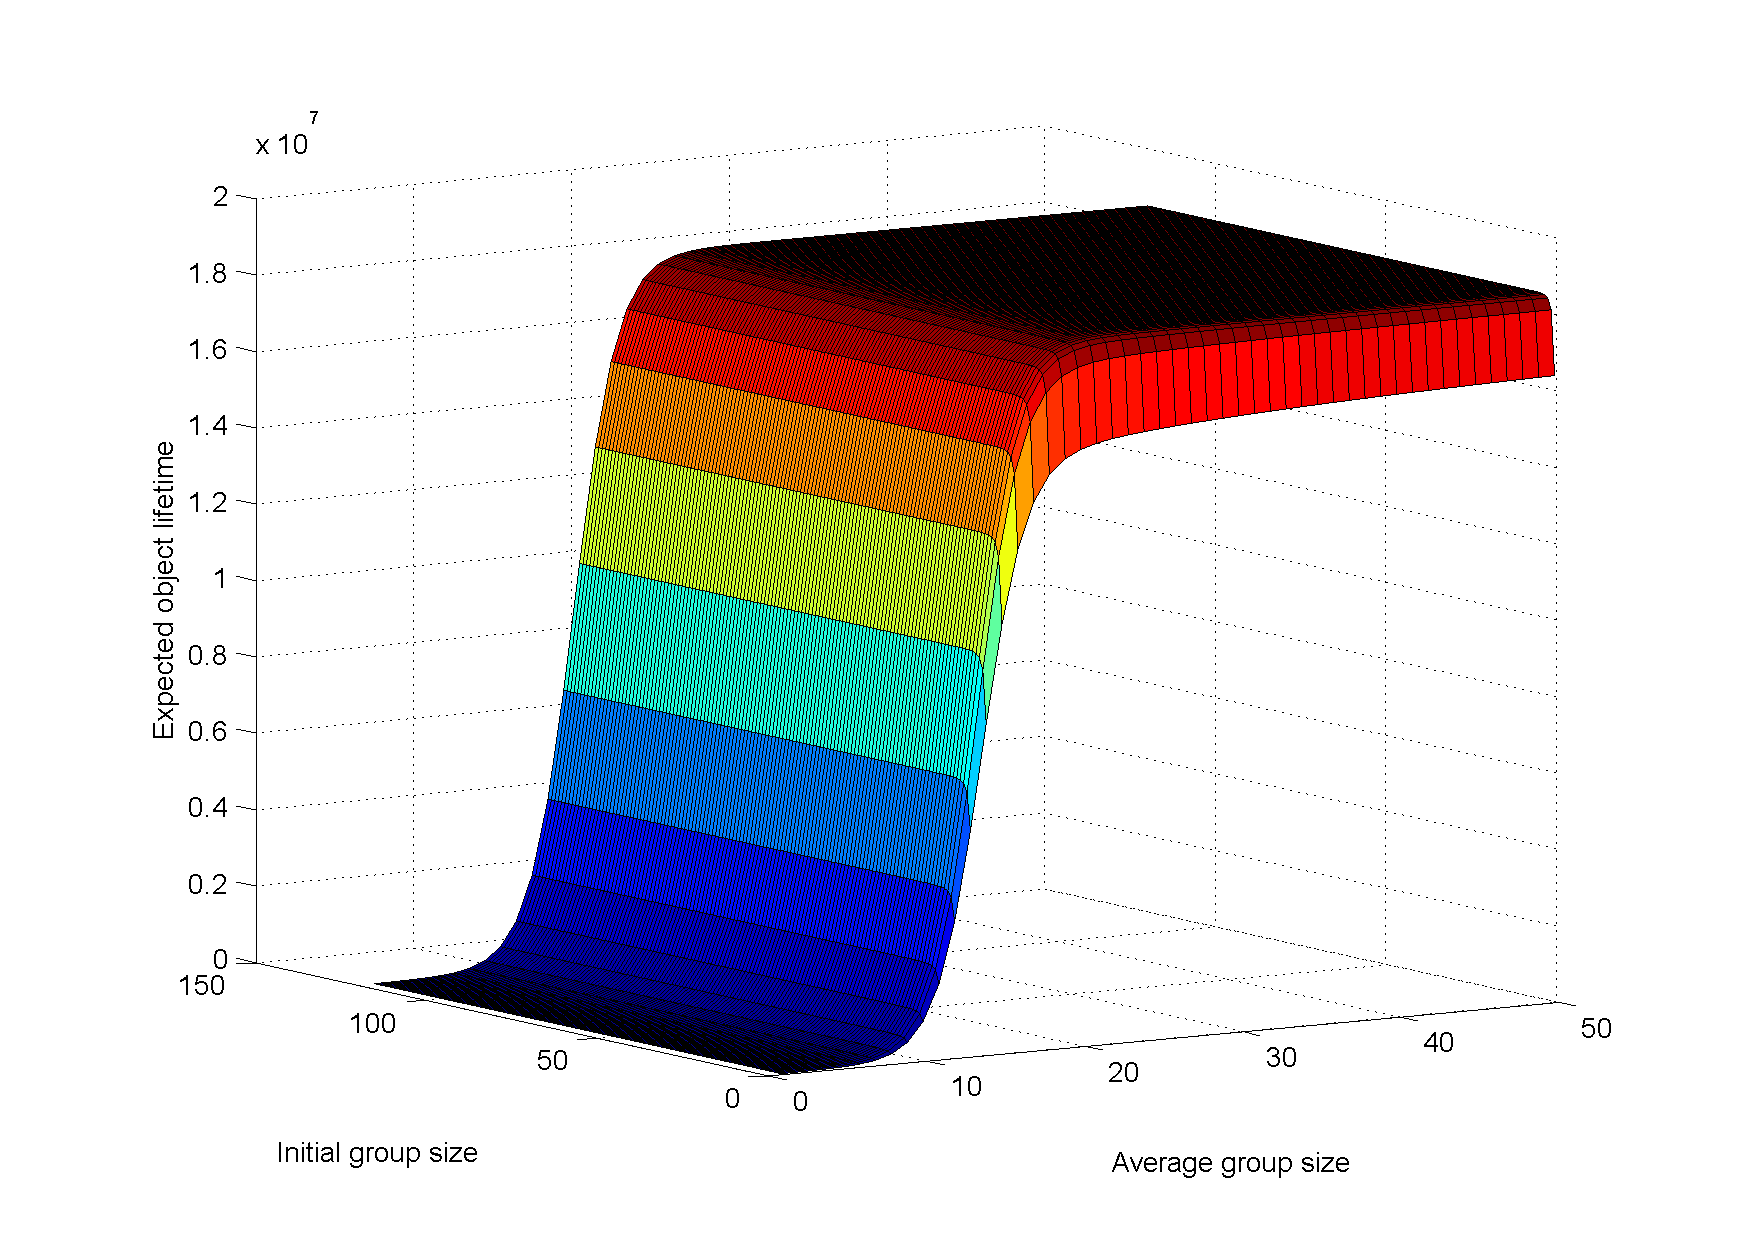
\includegraphics[clip=true, viewport=1.5cm 3.5cm 28.0cm 16.5cm, width=\columnwidth]{lifetime_av_init_groupsize}
 \caption{Surface plots of expected object lifetimes as functions of initial and average network sizes for $\mu = 1/180$ (above) and $\mu = 0$ (below).}
 \label{fig_lifetime_average_vs_initial}
\end{figure}
%
Figure \ref{fig_lifetime_average_vs_initial} shows surface plots of expected object lifetimes against initial and average network sizes for a repair rate of $\mu = 1/180$ (or $T_{\textrm{repair}}$ $10\%$ of the expected node lifetime) and no repair rate. It is evident that object lifetimes decrease greatly for average network sizes smaller than 20 nodes for the case with repair, but that average network size has no effect when repair is not used. The model presented in this chapter shows a significant decrease in expected lifetime every time the average network size is comparable to the required number of replicas, for the case with repair. The figure also shows that expected object lifetimes decrease when the initial network size is smaller than the required number of replicas. From the figure it can also be seen that initial network size has a more pronounced effect on the expected object lifetime, when no repair is used than when repair is used.

\begin{figure}[htbp]
 \centering
 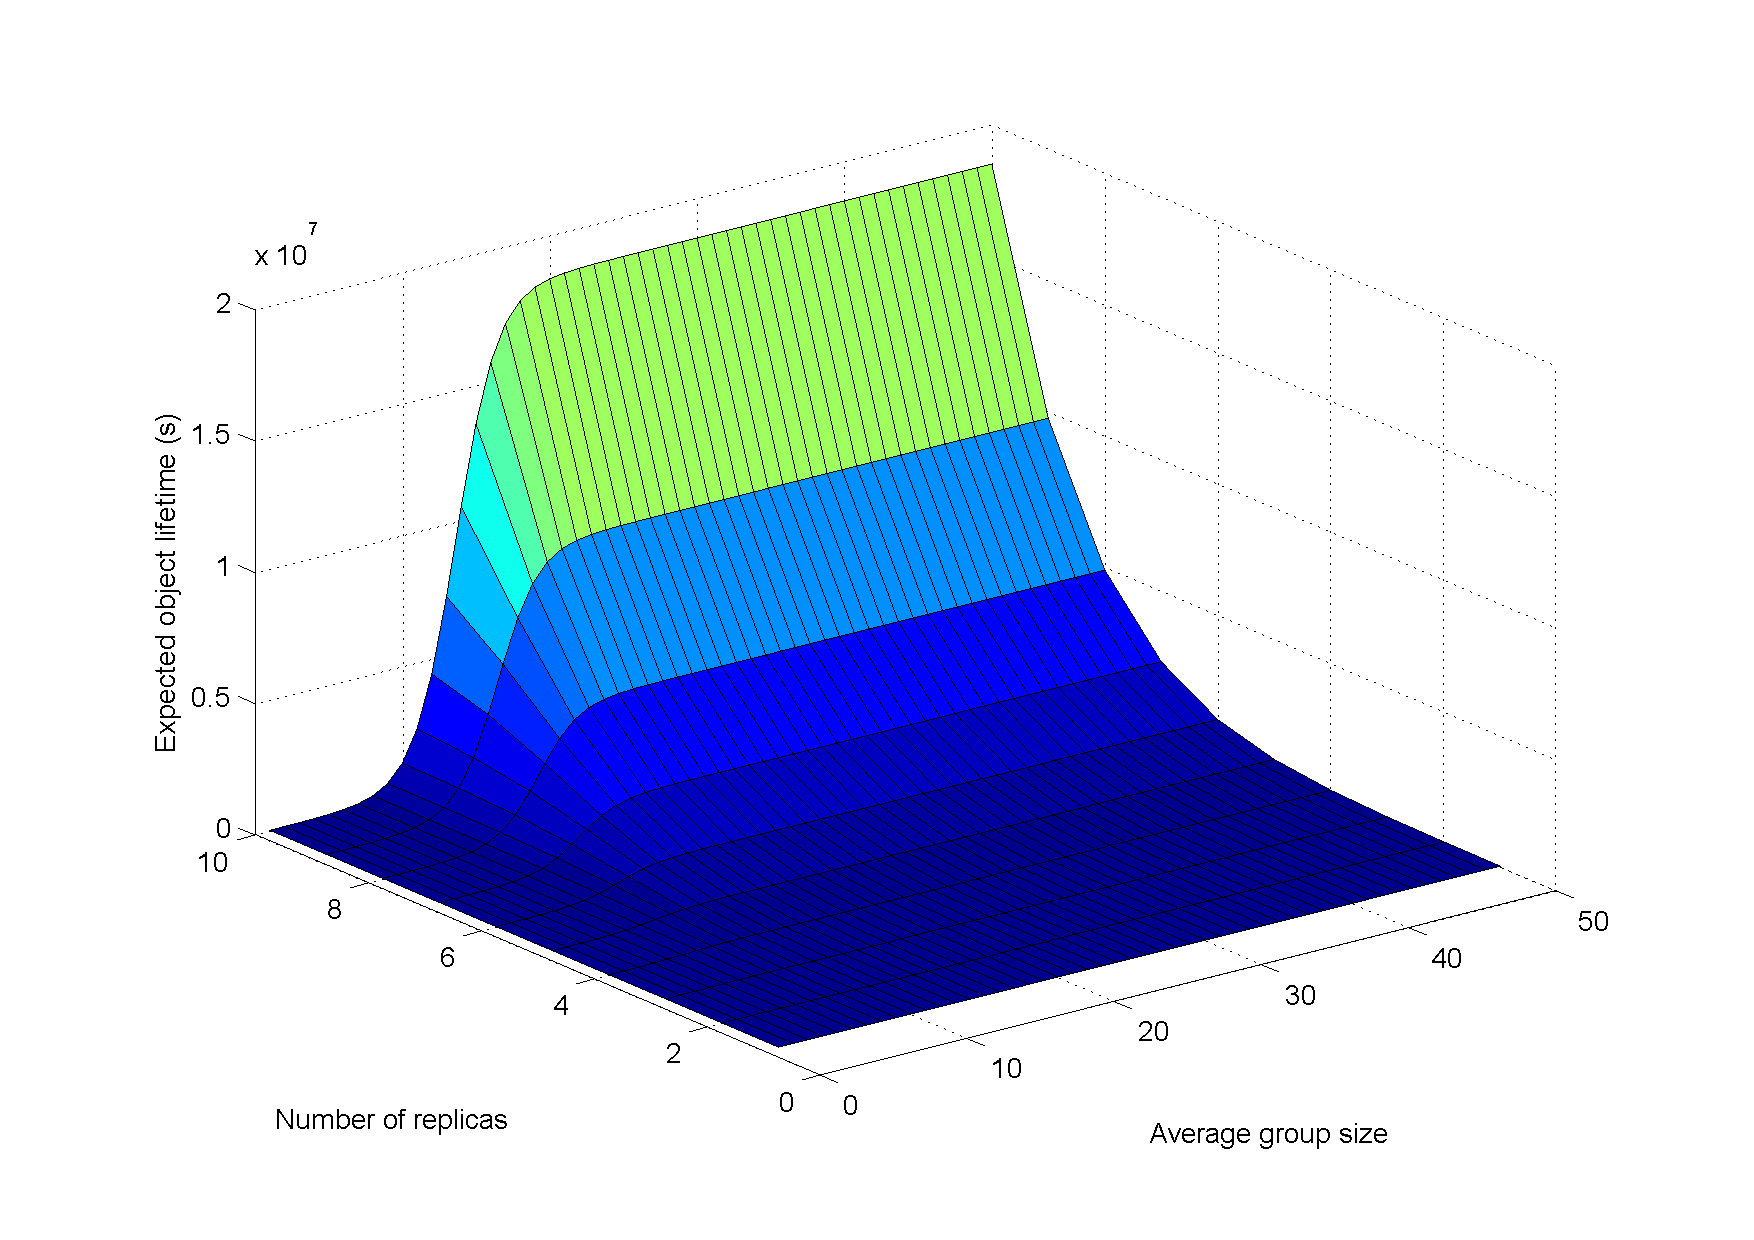
\includegraphics[clip=true, viewport=2.5cm 1.0cm 27.5cm 19.15cm, width=0.8\columnwidth]{lifetime_replicas_av_groupsize}
 \caption{Surface plot of expected object lifetimes as functions of average network size and required number of replicas $R$ for $mu = 1/180$.}
 \label{fig_lifetime_average_vs_replicas}
\end{figure}
%
Figure \ref{fig_lifetime_average_vs_replicas} depicts the expected object lifetime as functions of average network size and required number of replicas $R$ for a repair rate of $\mu = 1/180$. To generate this figure, $R$ is swept from 1 to 10 to illustrate the effect that an increase in the number of replicas has on the expected node lifetime. The figure shows that an increase in $R$ leads to an exponential increase in the expected object lifetime, but that this gain is limited when the average network size is small, compared to the required number of replicas.

\begin{figure}[htbp]
 \centering
 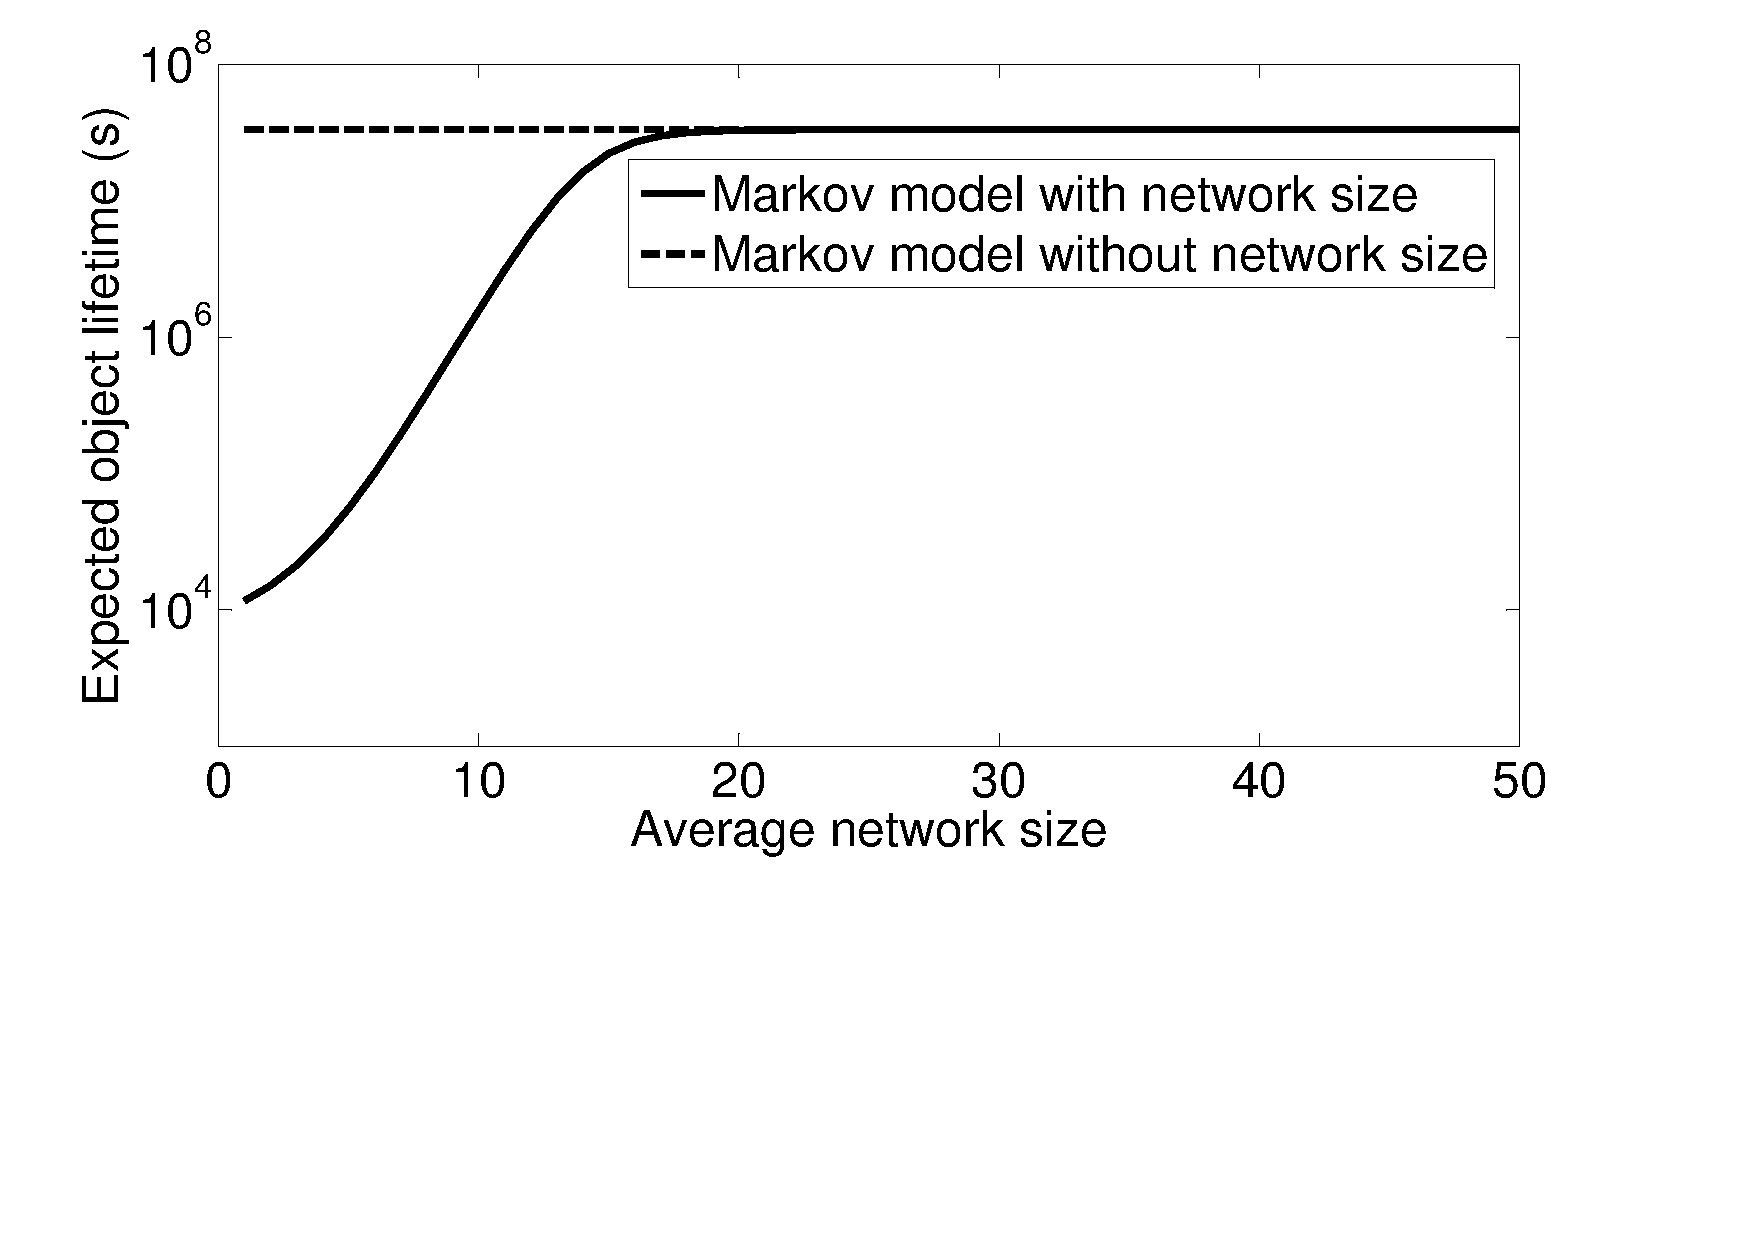
\includegraphics[clip=true, viewport=1.0cm 6.5cm 26.5cm 20.5cm, width=0.8\columnwidth]{lifetime_av_models_compare}
 \caption{Surface plot of expected object lifetimes as functions of initial and average group sizes.}
 \label{fig_lifetime_vs_other_model}
\end{figure}

Figure \ref{fig_lifetime_vs_other_model} compares the model presented in this chapter with the model of Wu, Tian and Ng that assumes object repair \cite{replication_article}. For this figure, a repair rate of $\mu = 1/180$ and a required number of replicas of $R = 10$ were used. As shown, because the model by Wu, Tian and Ng does not take average network size into account (or initial network size for that matter) it cannot predict the object lifetimes correctly for average network sizes comparable to the required number of replicas. On the other hand, a reliability test of the model presented in this chapter is that for sufficiently large network sizes, the model converges to the model that assumes an infinite network size.

\section{Comparison with Pithos simulation}
\label{simulation}

To determine practical usability of the theoretical results presented in Section \ref{results}, a comparison was performed against the Pithos simulation \cite{Pithos_mmve_2011}. Pithos is a hierarchical distributed storage system that uses grouping to reduce latencies of store and retrieve requests, as is required by massively multi-user virtual environments (MMVEs) \cite{gilmore_p2p_mmog_state_persistency}.

The Oversim environment contains churn generators that create \emph{peers} with lifetimes sampled from an exponential distribution. A single \emph{super peer} was also created and never destroyed. Super peers allow new nodes to join the group by working with the dedicated \emph{directory server} for network bootstrapping. A single group was used, because multiple groups have different average group sizes during different simulations, which reduces the number of measurements per average group size to below statistical significance.

During a simulation run, the Pithos test application generates random objects and require these objects to be stored in the network. Every node only generated objects for a specified amount of time. This is done to limit the total number of objects present in the system to a few hundred thousand. For numbers larger than this, the simulation would run out of memory and grind to a halt. To allow simulation of the case of long lived objects, the Pithos simulation was deployed on a ``High-Memory Quadruple Extra Large Instance'' in the Amazon EC2 cloud, which contains 68.4 GB of RAM.

``Box and whiskers plots'' are used to compare the simulation data with the theoretical model. This allows for comparisons of mean values, but also shows how the data are distributed. In the box plot, the black striped whiskers show the minima and maxima of the data sets. The lower and upper bounds of the boxes show the 25th and 75th percentiles respectively. The horizontal lines in the boxes show the medians of the data, and the ``notches'' around the medians show the 5\% significance levels. The cross present in every box shows the simulation data mean and the solid line running through the boxes shows expected object lifetimes as predicted by the theoretical model.

\begin{figure}[htbp]
 \centering
 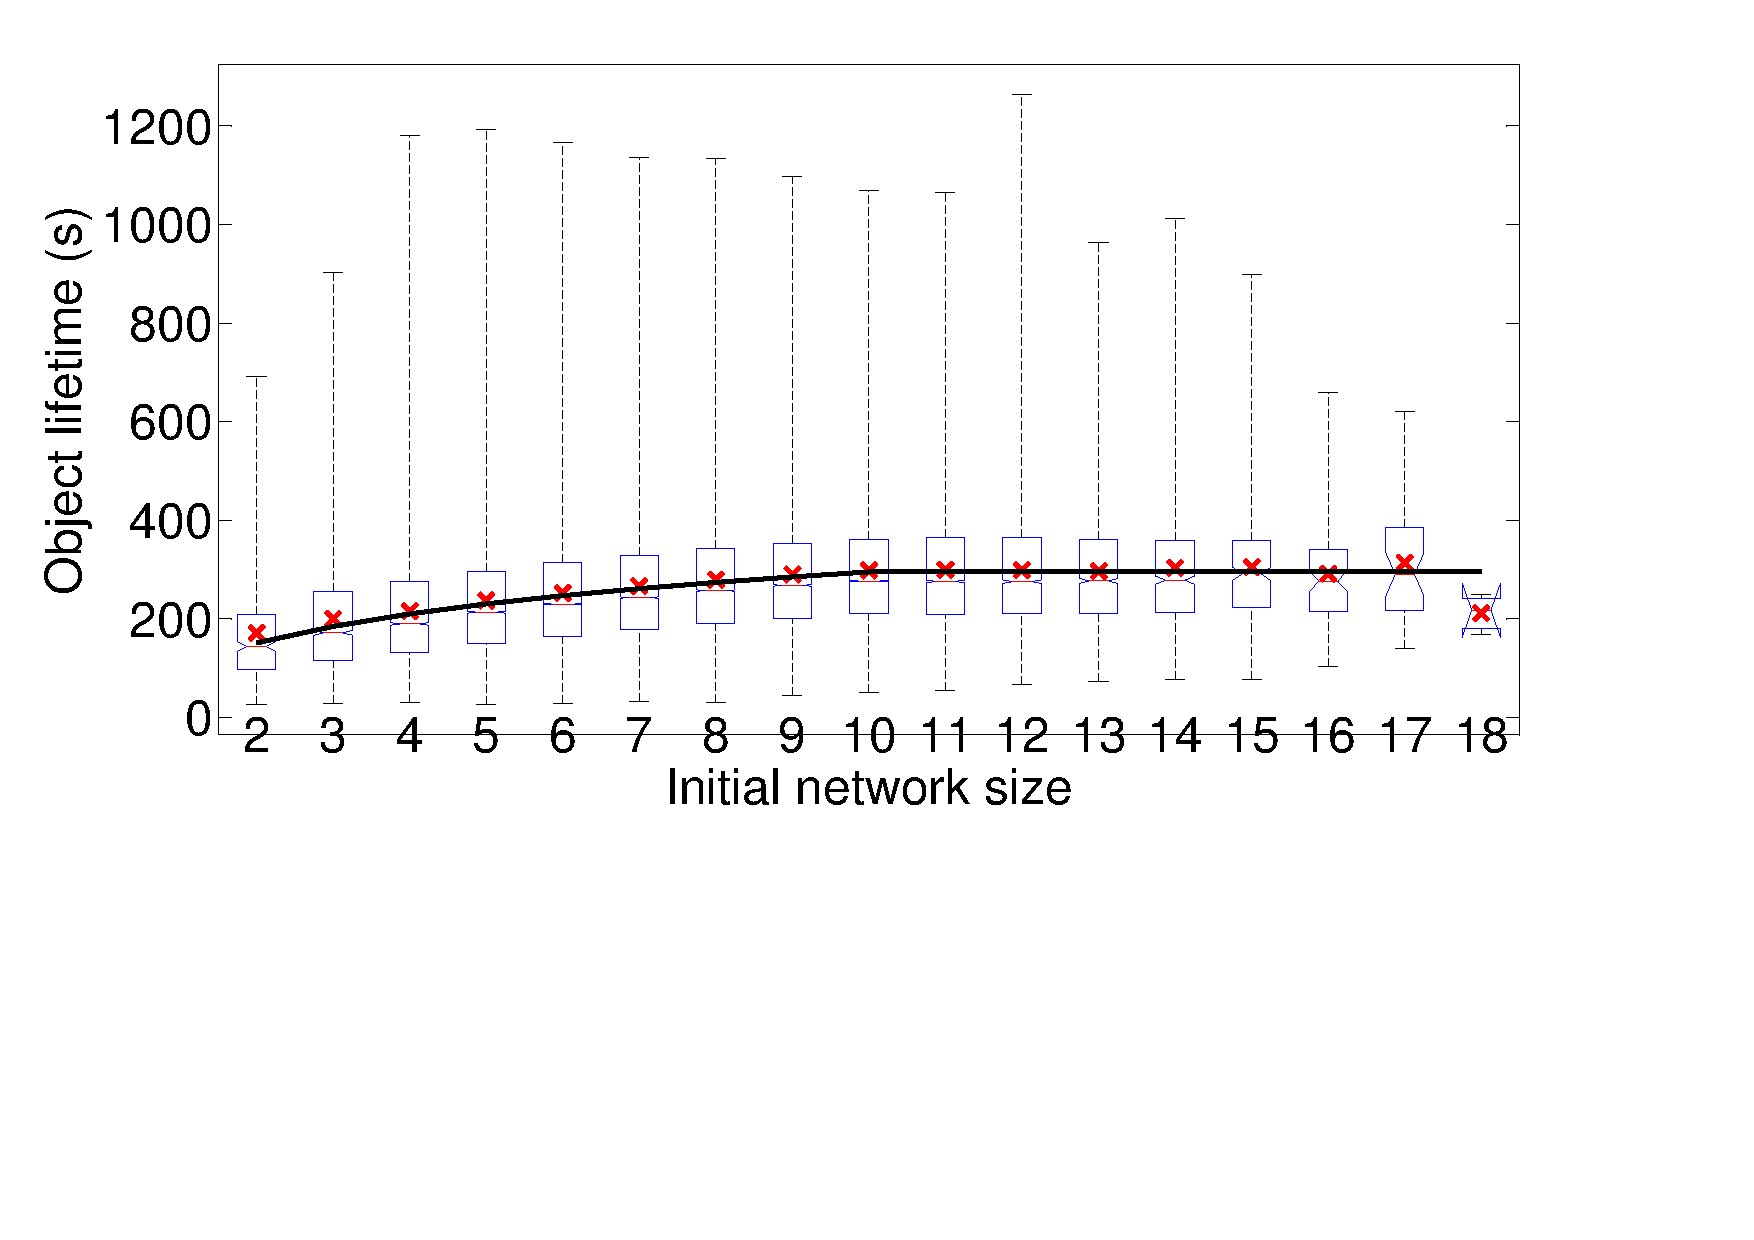
\includegraphics[clip=true, viewport=0.5cm 7.0cm 26.0cm 20.0cm, width=\columnwidth]{lifetime_simulation_model_none_100}
 \caption{Comparison of object lifetime simulation results, as a box plot, with theoretical model results for no repair, node lifetimes of $100 s$ and an average network size of 7 nodes.}
 \label{fig_lifetime_simulation_model_none_100}
\end{figure}
%
Figure \ref{fig_lifetime_simulation_model_none_100} compares the theoretical results to simulation results for the case where no repair is performed. Node have expected lifetimes of $100 s$, the number of required replicas are 10 nodes and the average network size is 7 nodes.

The expected object lifetimes as predicted by the theoretical model pass through the crosses that show the simulation data means. It can, therefore, be seen that the theoretical model matches the simulation data well for the case with no repair.

\begin{figure}[htbp]
 \centering
 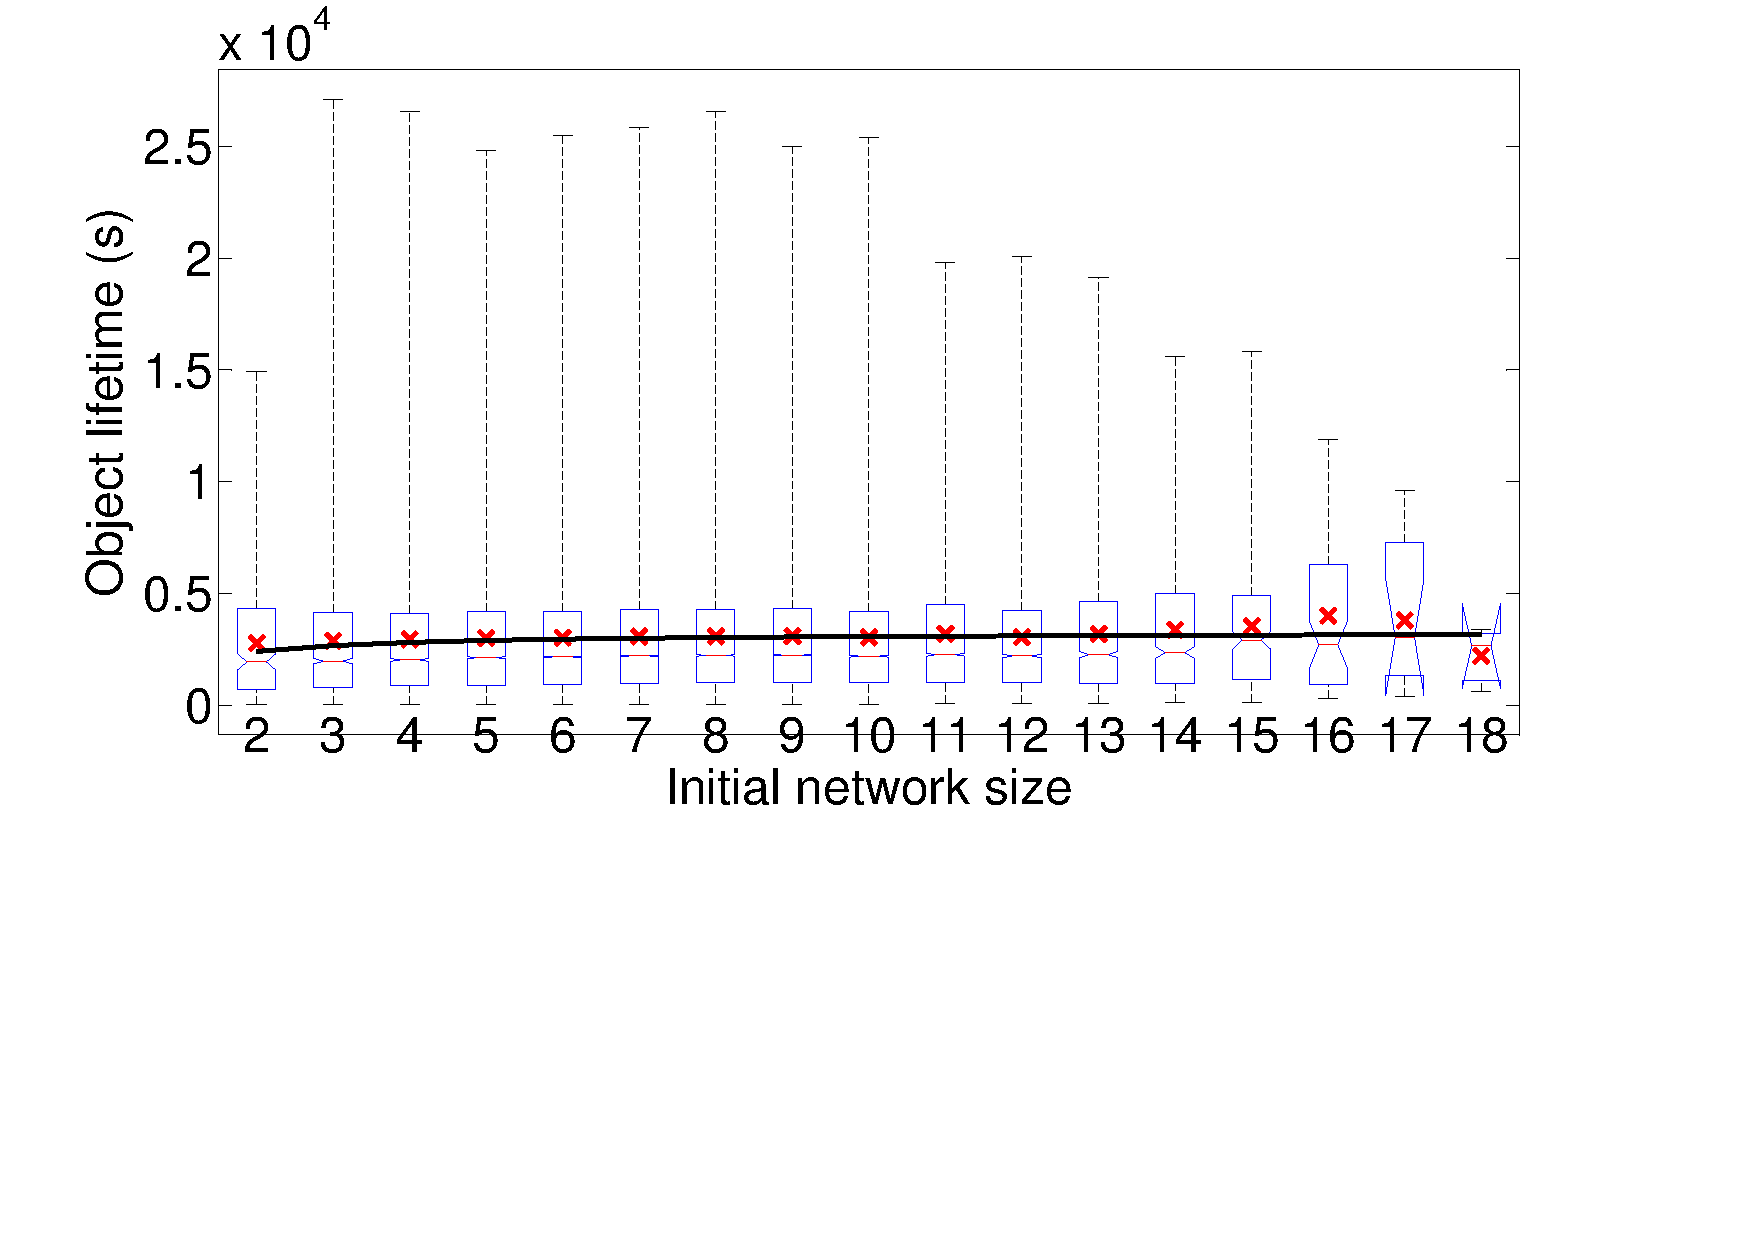
\includegraphics[clip=true, viewport=1.2cm 7.0cm 26.0cm 21cm, width=\columnwidth]{lifetime_simulation_model_20_100}
 \caption{Comparison of object lifetime simulation results, as a box plot, with theoretical model results for a repair time of $20 s$, node lifetimes of $100 s$ and an average network size of 7 nodes.}
 \label{fig_lifetime_simulation_model_20_100}
\end{figure}
%
Figure \ref{fig_lifetime_simulation_model_20_100} shows simulation data and theoretical model data for the same parameters as the previous figure, but for the case with $20 s$ repair time. A significant increase in object lifetimes can be observed. Again, the expected object lifetime as predicted by the model pass through the measured object lifetime means of the simulations. For initial network sizes on the edges of measured data, the simulation data might seem to deviate from the model data. However, in these ranges, only a few hundred measurements could be made, instead of the few thousand measurements made away from the maximum and minimum initial network size. The inaccuracy in these ranges can also be seen from the wide 5\% significance levels.

One issue that was encountered when comparing simulation data to model data was the imperfect repair scheme used in simulation. In the simulation, every $T_{\textrm{repair}}$ time, a repair of all objects in the system is initiated. In simulation, there is, however, a chance that the node that was chosen to repair an object leaves the network before the repair can complete. This reduces the effectiveness of the repair mechanism, reducing the effective repair rate. The percentage repair successes was measured during simulation and found to be $70 \%$. All repair rates in the simulation were adjusted with this number, which successfully aligned the simulation data means with the model data means.

\section{Conclusion}

A Markov chain that takes network size into account when predicting object lifetimes was presented. Results show that when the average network size is comparable to the required number of replicas, object lifetimes are significantly decreased. The theoretical model was shown to be equivalent to a model that ignores network size, when the average network size is large, compared to the required number of replicas. The model was also shown to compare well to simulation, with values being nearly equal.

We show how to reliably predict expected object lifetimes. When it is known that the average network size is comparable to the required number of replicas, the network size should be taken into account when modelling object lifetimes in a situation with repair. The theoretical model presented here allows for the design of a distributed storage system when the various average network sizes and node lifetime distributions are known.

Future work includes comparing object lifetimes using replication, with object lifetimes using erasure coding as redundancy technique. Modelling object lifetimes using heavy-tailed node lifetime distributions, such as the Pareto distribution, is also required. The variable failure rate of the Pareto distribution complicates modelling it as a Markov chain.
